\chapter{Simulations and Real Robot Experiments}
\label{ch:chapter_seven}%

The simulation environments and the robot hardware have been described in chapter \ref{ch:chapter_four}, and details on the different test environments were given in the previous chapter. 
The main focus of this research has been the implementation of the motion control system for GRIEEL joints, and the definition of the transformation algorithm (see chapter \ref{ch:chapter_five}). Here details on the validation setup are provided, both for simulation and for the real LIMBERO-GRIEEL robotic system. 

The performance verification workflow is described first for the simulation environment, then for the single limb, and Finally for the overall robot in the laboratory. 
The results are discussed in the next chapter, both quantitatively and qualitatively. 

Furthermore, some hardware limitations, identified during single limb tests and whole robot setup, are discussed in this chapter. 

\section{Simulations with Gazebo}
\label{sec:simulation}

The two simulation environments have been used in different stages of the research and for different purposes. Here, the tests performed and the main objectives are discussed. 

\subsection{Gazebo Classic}
\label{sec:gz_classic}

Gazebo Classic is used to test the extension of the multi-layer robot control software from the 4-DOF to the 7-DOF LIMBERO-GRIEEL robot. Here, the module transformation is not implemented (open/close the finger), and motion tasks for GRIEEL are tested in terms of wrist and driving joint control.

The importance of this initial simulation setup has been already discussed in this thesis. 
In synthesis it has been fundamental for: 
\begin{itemize}
    \setlength\itemsep{-0.7em} 
    \item \textbf{Software update}: testing the software to control GRIEEL's joints during the implementation.
    \item \textbf{Transformation algorithm implementation}: Developing the transition algorithm before real experiments.
    \item \textbf{Reliable physics computation}: Gazebo uses a physics engine that includes forces such as inertial effect, gravity, and friction, providing a realistic environment. In this way, even if a static stability criterion such as the SSM has been used to define base CoM positioning, it is possible to check stability under disturbances not considered. In particular, the GRIEEL joints' motion during the transition creates additional dynamical effects, that in principle can destabilize the robot. Using Gazebo it was possible to test this disturbances both for the transition algorithm and for the basic motion controller. 
\end{itemize}

The mistake that was made when setting up this simulator was an oversizing of the feasible joint effort (torque) from the real motor's rated torque. This aspect was a problem during the experiments and has been considered in the migration to the newer version of the simulator, to set up a more reliable real-to-sim environment.  

Furthermore, a big problem of Gazebo Classic is the setup of contact and dissipative forces parameters, small changes lead to unrealistic behavior, penetration of collision elements, and model "explosions". After some empirical comparison, it was noticed that using the newer version of Gazebo (Harmonic) ensures better physical stability, without excessive effort to update the software. 

\subsection{Gazebo Harmonic}
\label{sec:gz_harmonic}

As already mentioned, the need to set up a new simulator stems from the inability to access the robot hardware.
Here also finger joints are integrated and controlled, to perform complete transformation experiments and additional complex motion tasks.
In this new environment, the problem of feasible motors' torque has been considered, and complex motion sequences not possible with the real hardware (as discussed in the next) have been tested: 

\begin{itemize}
    \setlength\itemsep{-0.7em} 
    \item \textbf{IJCs implementation}: The new low-level control infrastructure implemented from scratch is tested.
    \item \textbf{Locomotion execution}: The ability to perform both a simple crawl gait walking and a driving forward locomotion is addressed and analyzed.
    \item \textbf{Locomotion transition}: The transformation of all GRIEEL modules from G2W and vice versa is further investigated.
    \item \textbf{Complex locomotion}: Locomotion in hybrid configuration (3 wheels -1 gripper) is tested. 
\end{itemize}

\section{Single Limb Test Bench}
\label{sec:single_limb}

The transition from simulation to the real system requires verification of the operation of the control software implemented for the new limb structure.
Reliability and performance are first tested on a single limb, then assembling the quadruped LIMBERO-GRIEEL is possible. 

The setup used to ensure the system operation is a single-limb test bench (represented in Fig.\ref{fig:limb_testbench}). 
The main components of this basic test bench are: 
\begin{itemize}
    \setlength\itemsep{-0.7em} 
    \item \textbf{Emergency stop switch}
    \item \textbf{Gripping surface}: to test ground gripper performance.
    \item \textbf{Vertical linear rail}: fixed with an aluminum frame to test swing motions or free to slide and weighted to test supporting abilities. 
\end{itemize}

\begin{figure}[H]
    \centering
    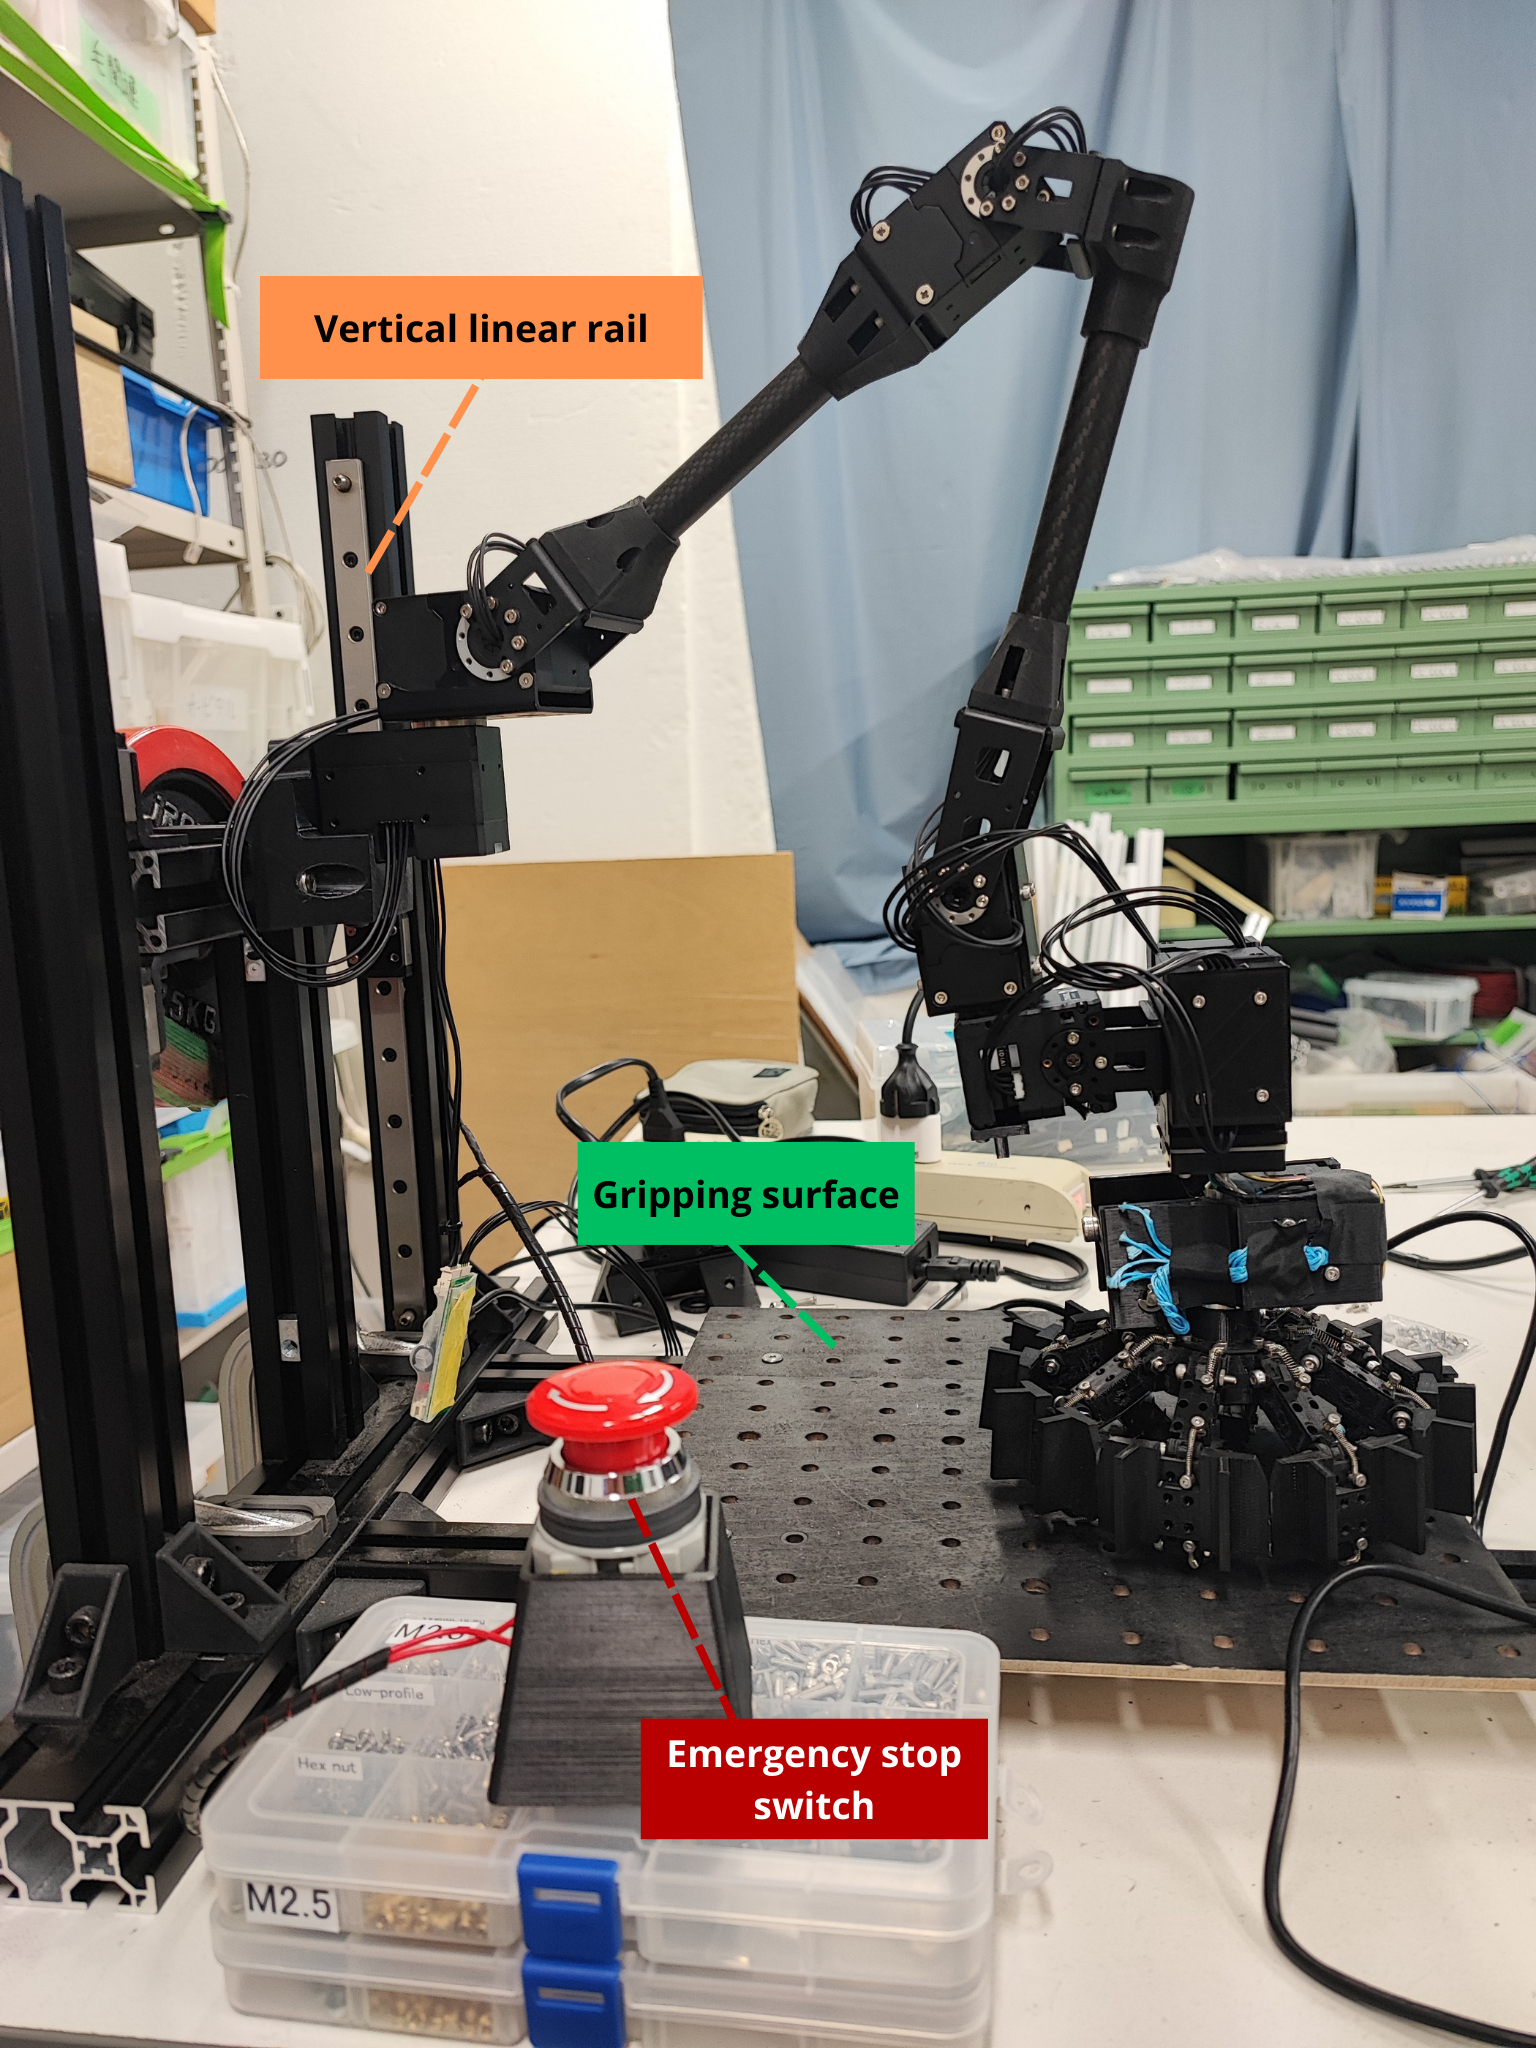
\includegraphics[width=0.45\textwidth]{Images/img_ch7/single_limb_testbench.png}
    \caption{Single Limb testbench}
    \label{fig:limb_testbench}
\end{figure}

In this safe environment, the following operations have been conducted before the final experiments: 
\begin{enumerate}
    \setlength\itemsep{-0.7em} 
    \item\label{item:limbtest_1} Configure DYNAMIXEL motors.
    \item\label{item:limbtest_2} Test single limb motion control
    \item\label{item:limbtest_3} Adjust servomotors gains (as discussed in \ref{sec:dynamixel_motors})
    \item\label{item:limbtest_4} Verify the ability of the motors to counteract GRIEEL weight.
    \item\label{item:limbtest_5} Integrate additional locking motors commands and timing to lbr\_dynamixel\_control, to open/close the gripper for transformation.
    \item\label{item:limbtest_6} Execute the complete sequence of tasks required for the transition algorithm, both as G2W and as W2G.
    \item\label{item:limbtest_7} Test driving motor operation in velocity control mode.
    \item\label{item:limbtest_8} Integrate a contact estimation technique at the software level.
\end{enumerate}

It is relevant to comment steps (\ref{item:limbtest_4}), (\ref{item:limbtest_5}), and (\ref{item:limbtest_8}).
Regarding weight counteracting tests (\ref{item:limbtest_4}), limitations on C2F (shoulder) and FT2 (elbow joint) have been evident, In configurations where GRIEEL's overall CoM is far from that joint, gravitational torque increases (due to a longer moment arm). 
This is also relevant when the limbs have to support the base, as discussed in the next section.

Some quantitative considerations of this aspect are discussed in the limitation section of the result chapter (\ref{sec:limitations}). For now, it is important to note that the design and motor sizing don't meet the requirements.

Another problem addressed during single-limb setup is the absence of important feedback information required for autonomous task execution. 
In particular, sensors to detect the state of GRIEEL mode (gripper/wheel) are not yet integrated, and neither are solutions to detect ground/environment contact of the limb EE. 

To estimate the state of the GRIEEL transformation module (\ref{item:limbtest_5}), both locking motor revolutions and timing with constant velocity commands have been tested, however, finger springs wear and fluctuations of motor velocity create uncertainties. Fine-tuning of opening/closing timed commands has been conducted to complete the experiments. 

As a final encountered limitation, the contact state estimation is crucial in the execution of the transition algorithm, due to the usage of contact points to estimate the support polygon. 
Different software solutions have been considered 
as a workaround, in particular, the works of A.De Luca for sensorless collision detection for safe human-robot cooperation have been analyzed for a possible extension\cite{AdeLuca_sensorlesscollision1}\cite{AdeLuca_sensorlesscollision2}\cite{AdeLuca_sensorlesscollision3}\cite{AdeLuca_sensorlesscollision4}\cite{AdeLuca_sensorlesscollision5}. 
Also proprioceptive sensor filtering, in the context of legged robot locomotion provides useful insights
\cite{LeggedRobotStateEstimator}
\cite{ProprioceptiveSensorFusion}
\cite{EKFcontact}. Many of the solutions considered account not only for contact detection but for a complete force contact estimation, which was out of this research scope and more than the experiment requirements(contact detection). 
For this reason, two approaches have been used, but the second one was the only "reliable" workaround to complete the transition sequence: 
\begin{enumerate}
    \setlength\itemsep{-0.7em} 
    \item\label{item:contact_1} \textbf{Current based estimation}: Looking at the condition represented in Fig.\ref{fig:contact_estimation}, when a limb is in contact, the torque at C2F joint has to be positive to support the base. This corresponds to a positive electric current, which can be monitored from DYNAMIXEL interface. Using a simple approach similar to \cite{ContactCurrent}, from the current feedback, a current threshold has been defined to identify contacts. 
    \item\label{item:contact_2} \textbf{limb command assumption}: This approach is reliable only for the simple support plane condition tested in the laboratory, and under the assumption that limb tasks are executed correctly. When a limb translation task with positive z is sent, the contact state is false, while true for the equivalent negative z translation.  
    The limitations of this approach for any unstructured environments or unexpected base translation are clear. However, During the testing of the transformation algorithm motions and environment states are known, then this can be considered a valid approach. 
\end{enumerate}

\begin{figure}[H]
    \centering
    \subfloat[Limb in contact state, positive current (torque)\label{fig:contact}]{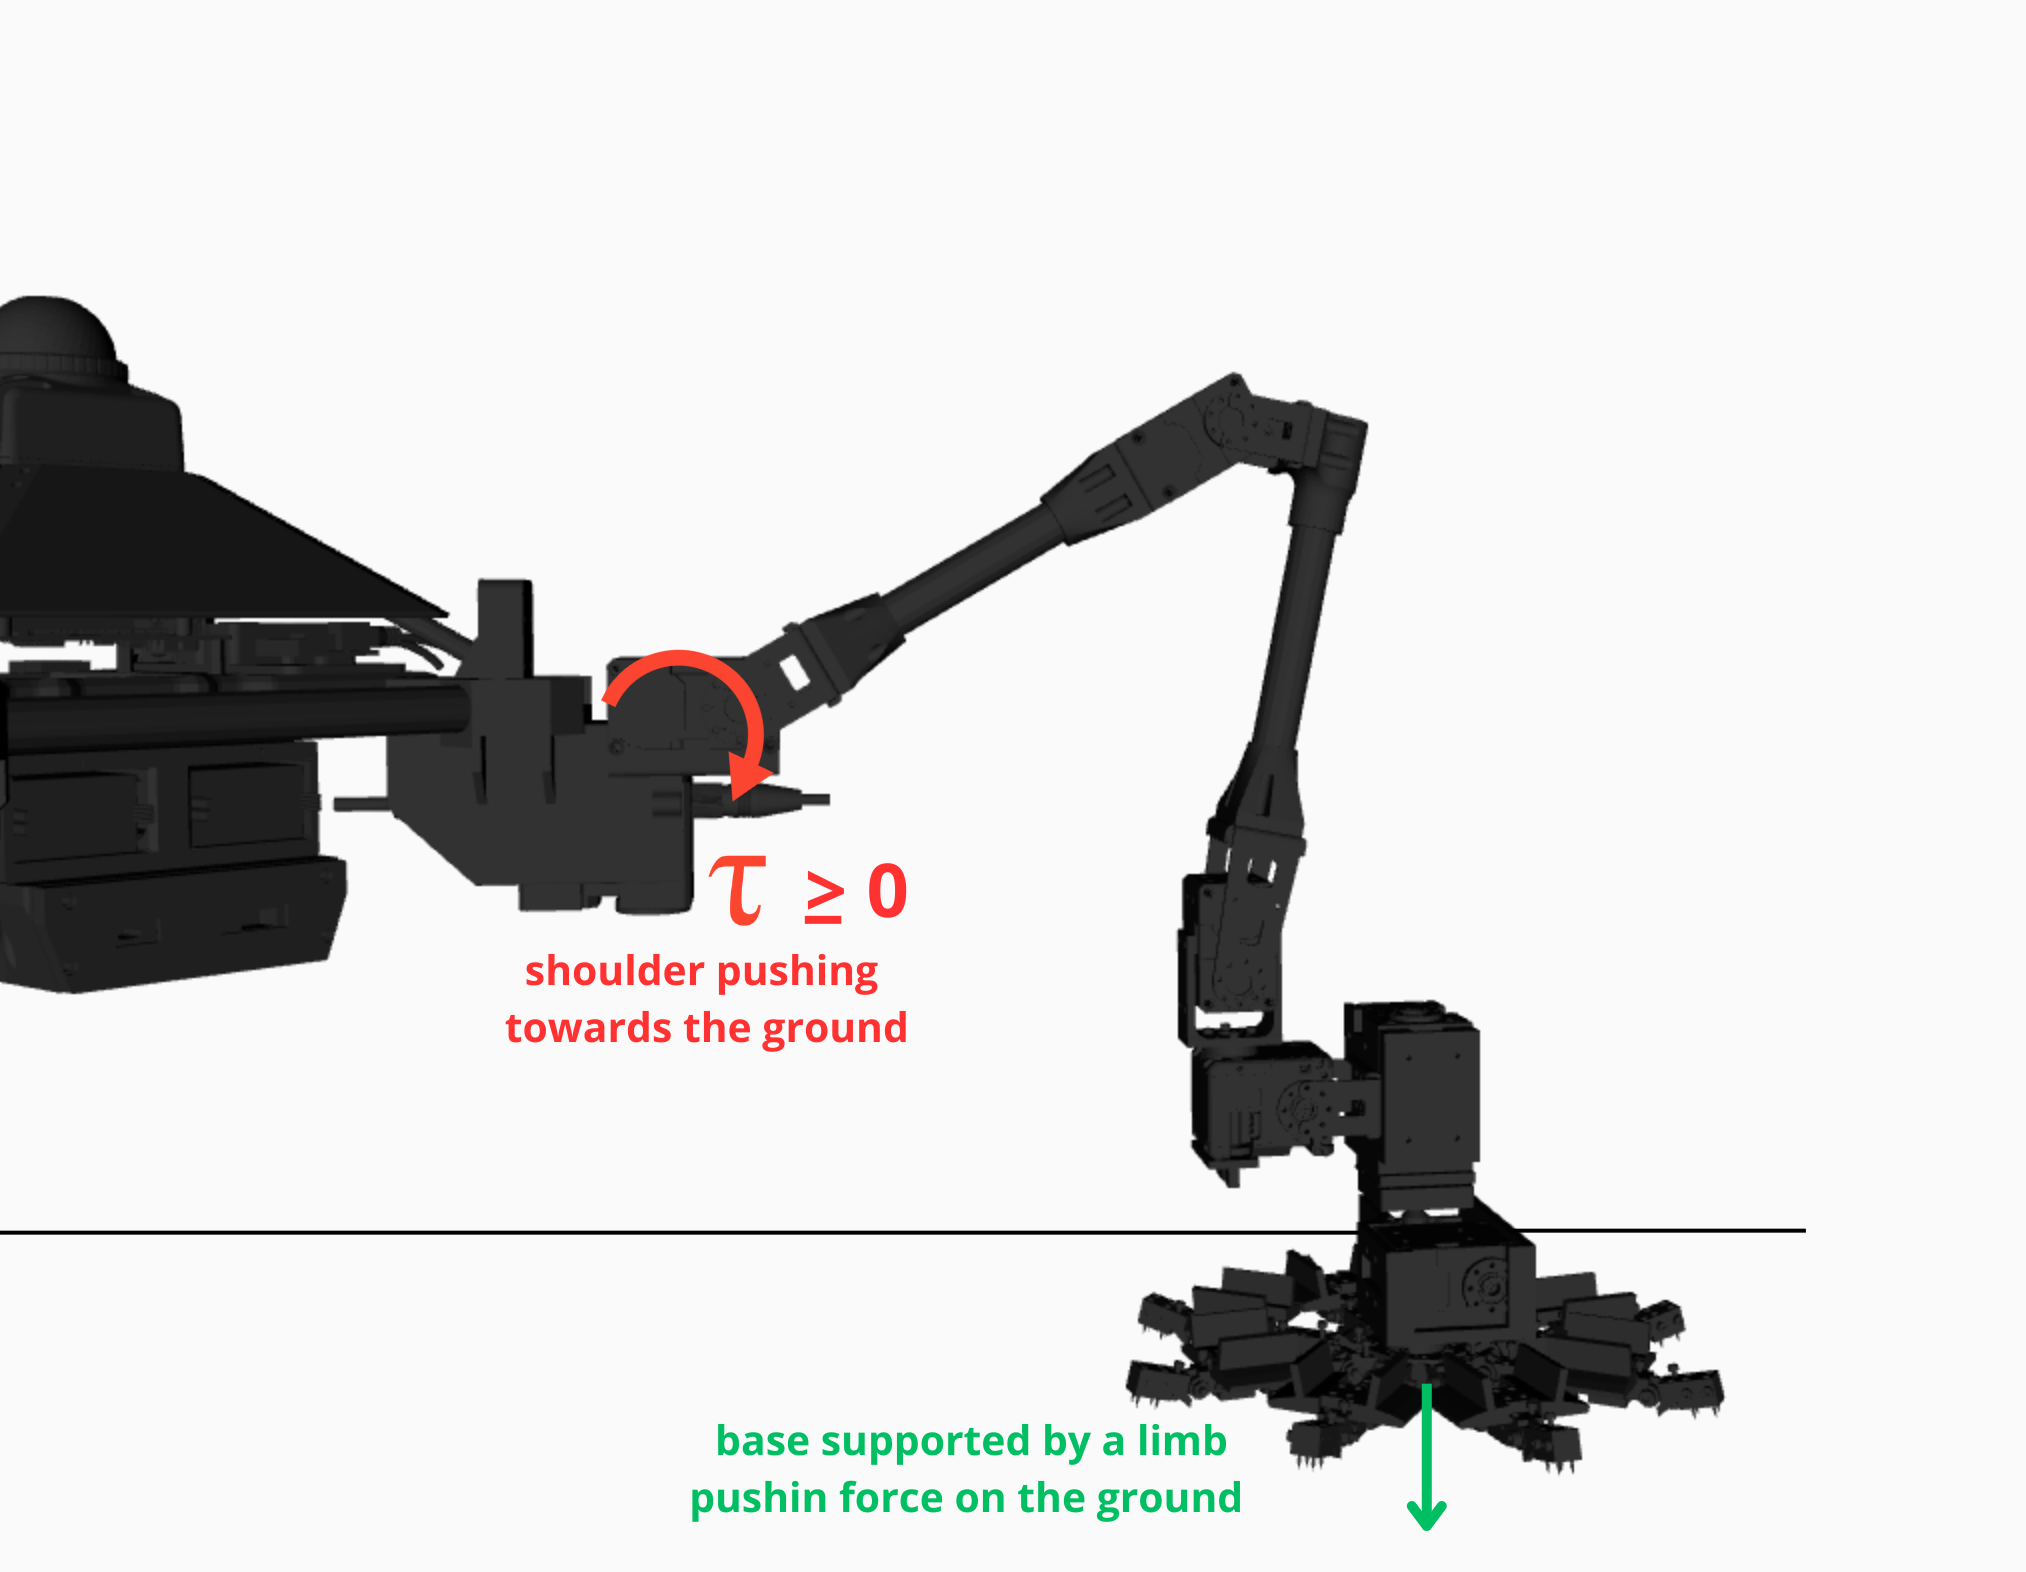
\includegraphics[width=0.45\textwidth]{Images/img_ch7/contact_torque.png}} \quad 
    \subfloat[Limb in swing state, negative current (torque)\label{fig:not_contact}]{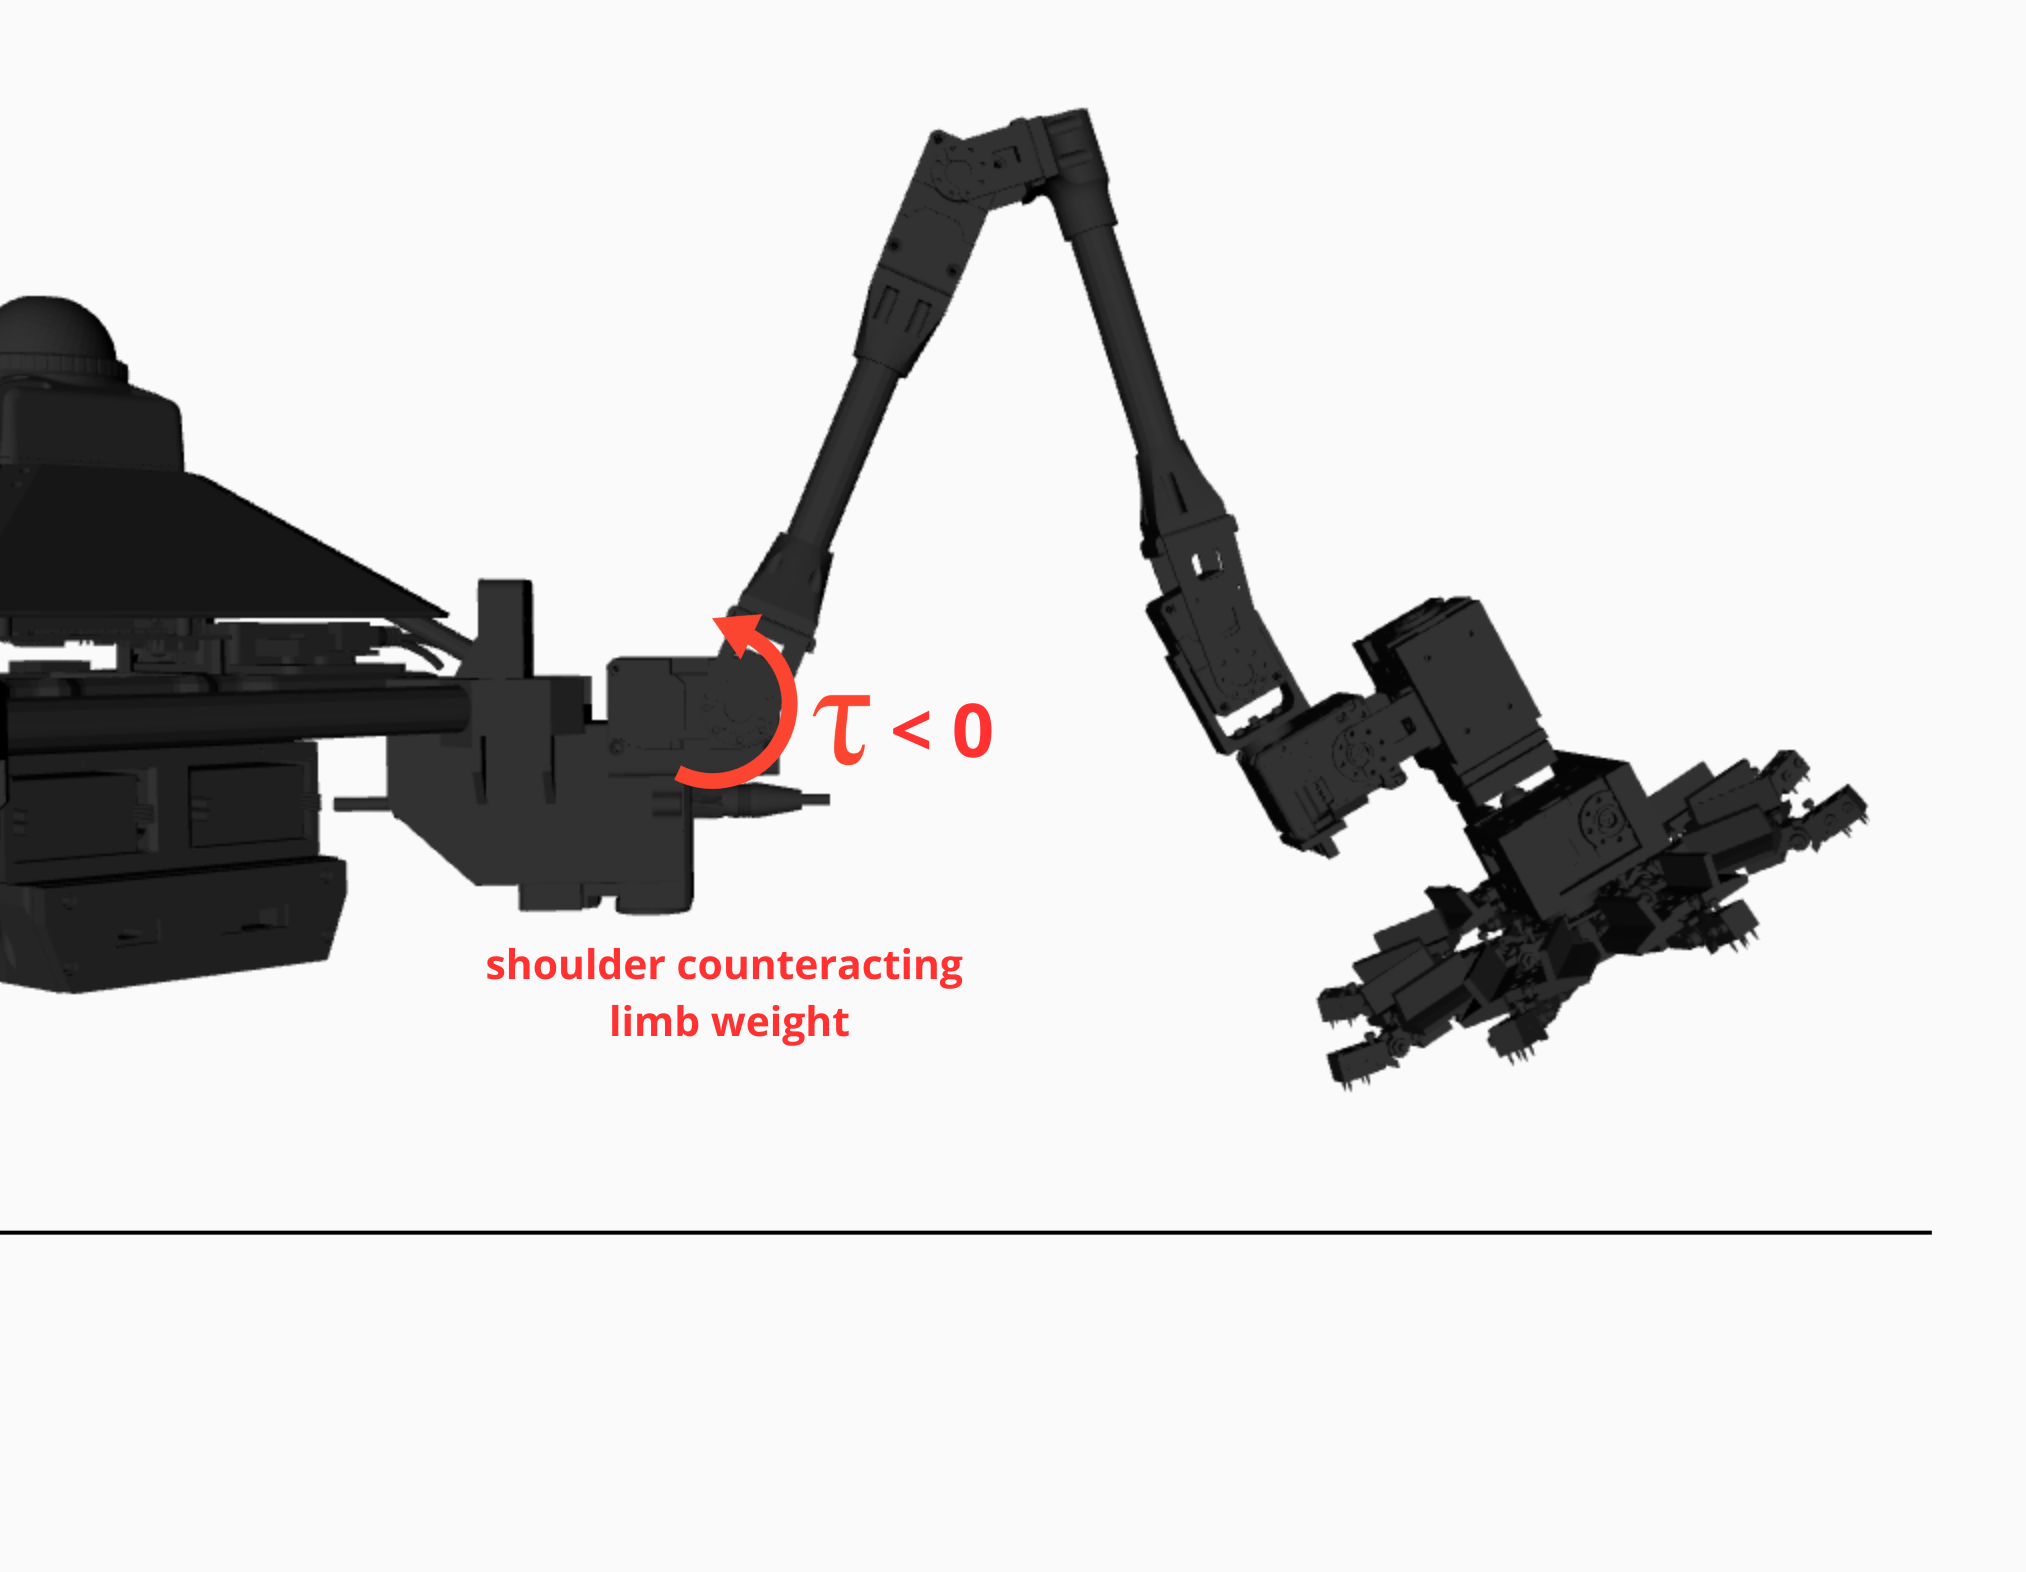
\includegraphics[width=0.45\textwidth]{Images/img_ch7/swing_torque.png}} 

    \caption[Schematic representation of current based contact estimation]{Schematic representation of current based contact estimation}
    \label{fig:contact_estimation}
\end{figure}

Multiple tests and implementations to integrate solution (\ref{item:contact_1}) has contact estimator has been done, but then on the whole robot often wrong estimations occur. For this reason, a simpler approach (\ref{item:contact_2}) has been implemented to complete the transformation algorithm.

It is evident that to test an adaptable autonomous motion sequence such as the one defined here, this simple approach is fine, but it is evident the necessity of integrating better contact estimations or even hardware solutions\cite{hapticcontact}\cite{WheelLeggedContact}.

Once the above limitations are solved in view of the experiments to be conducted on the LIMBERO-GREIEEL robot, and the reliability of limb control is ensured, the four limbs can be assembled into the robot base. 

\section{LIMBERO-GRIEEL Trasformation}
\label{sec:limbero_grieel_setup}

From the previous tests, The working condition of the single limbs has been proven, and the encountered limitations accounted for. First, the robot is assembled, and the following preliminary tests are conducted: 

\begin{enumerate}
    \setlength\itemsep{-0.7em} 
    \item\label{item:robot_test1} Test coordinated limb commands by supporting the base with an aluminum frame (as represented in Fig.\ref{fig:robot_testbench}). 
    \item\label{item:robot_test2} Verify the ability of four/three limbs to support the base without the aluminum frame, for different base heights and grieel modes.
    \item\label{item:robot_test4} Adjust DYNAMIXEL gains if needed. 
    \item\label{item:robot_test4} Perform additional tests on current-based contact state estimation. 
\end{enumerate} 

\begin{figure}[H]
    \centering  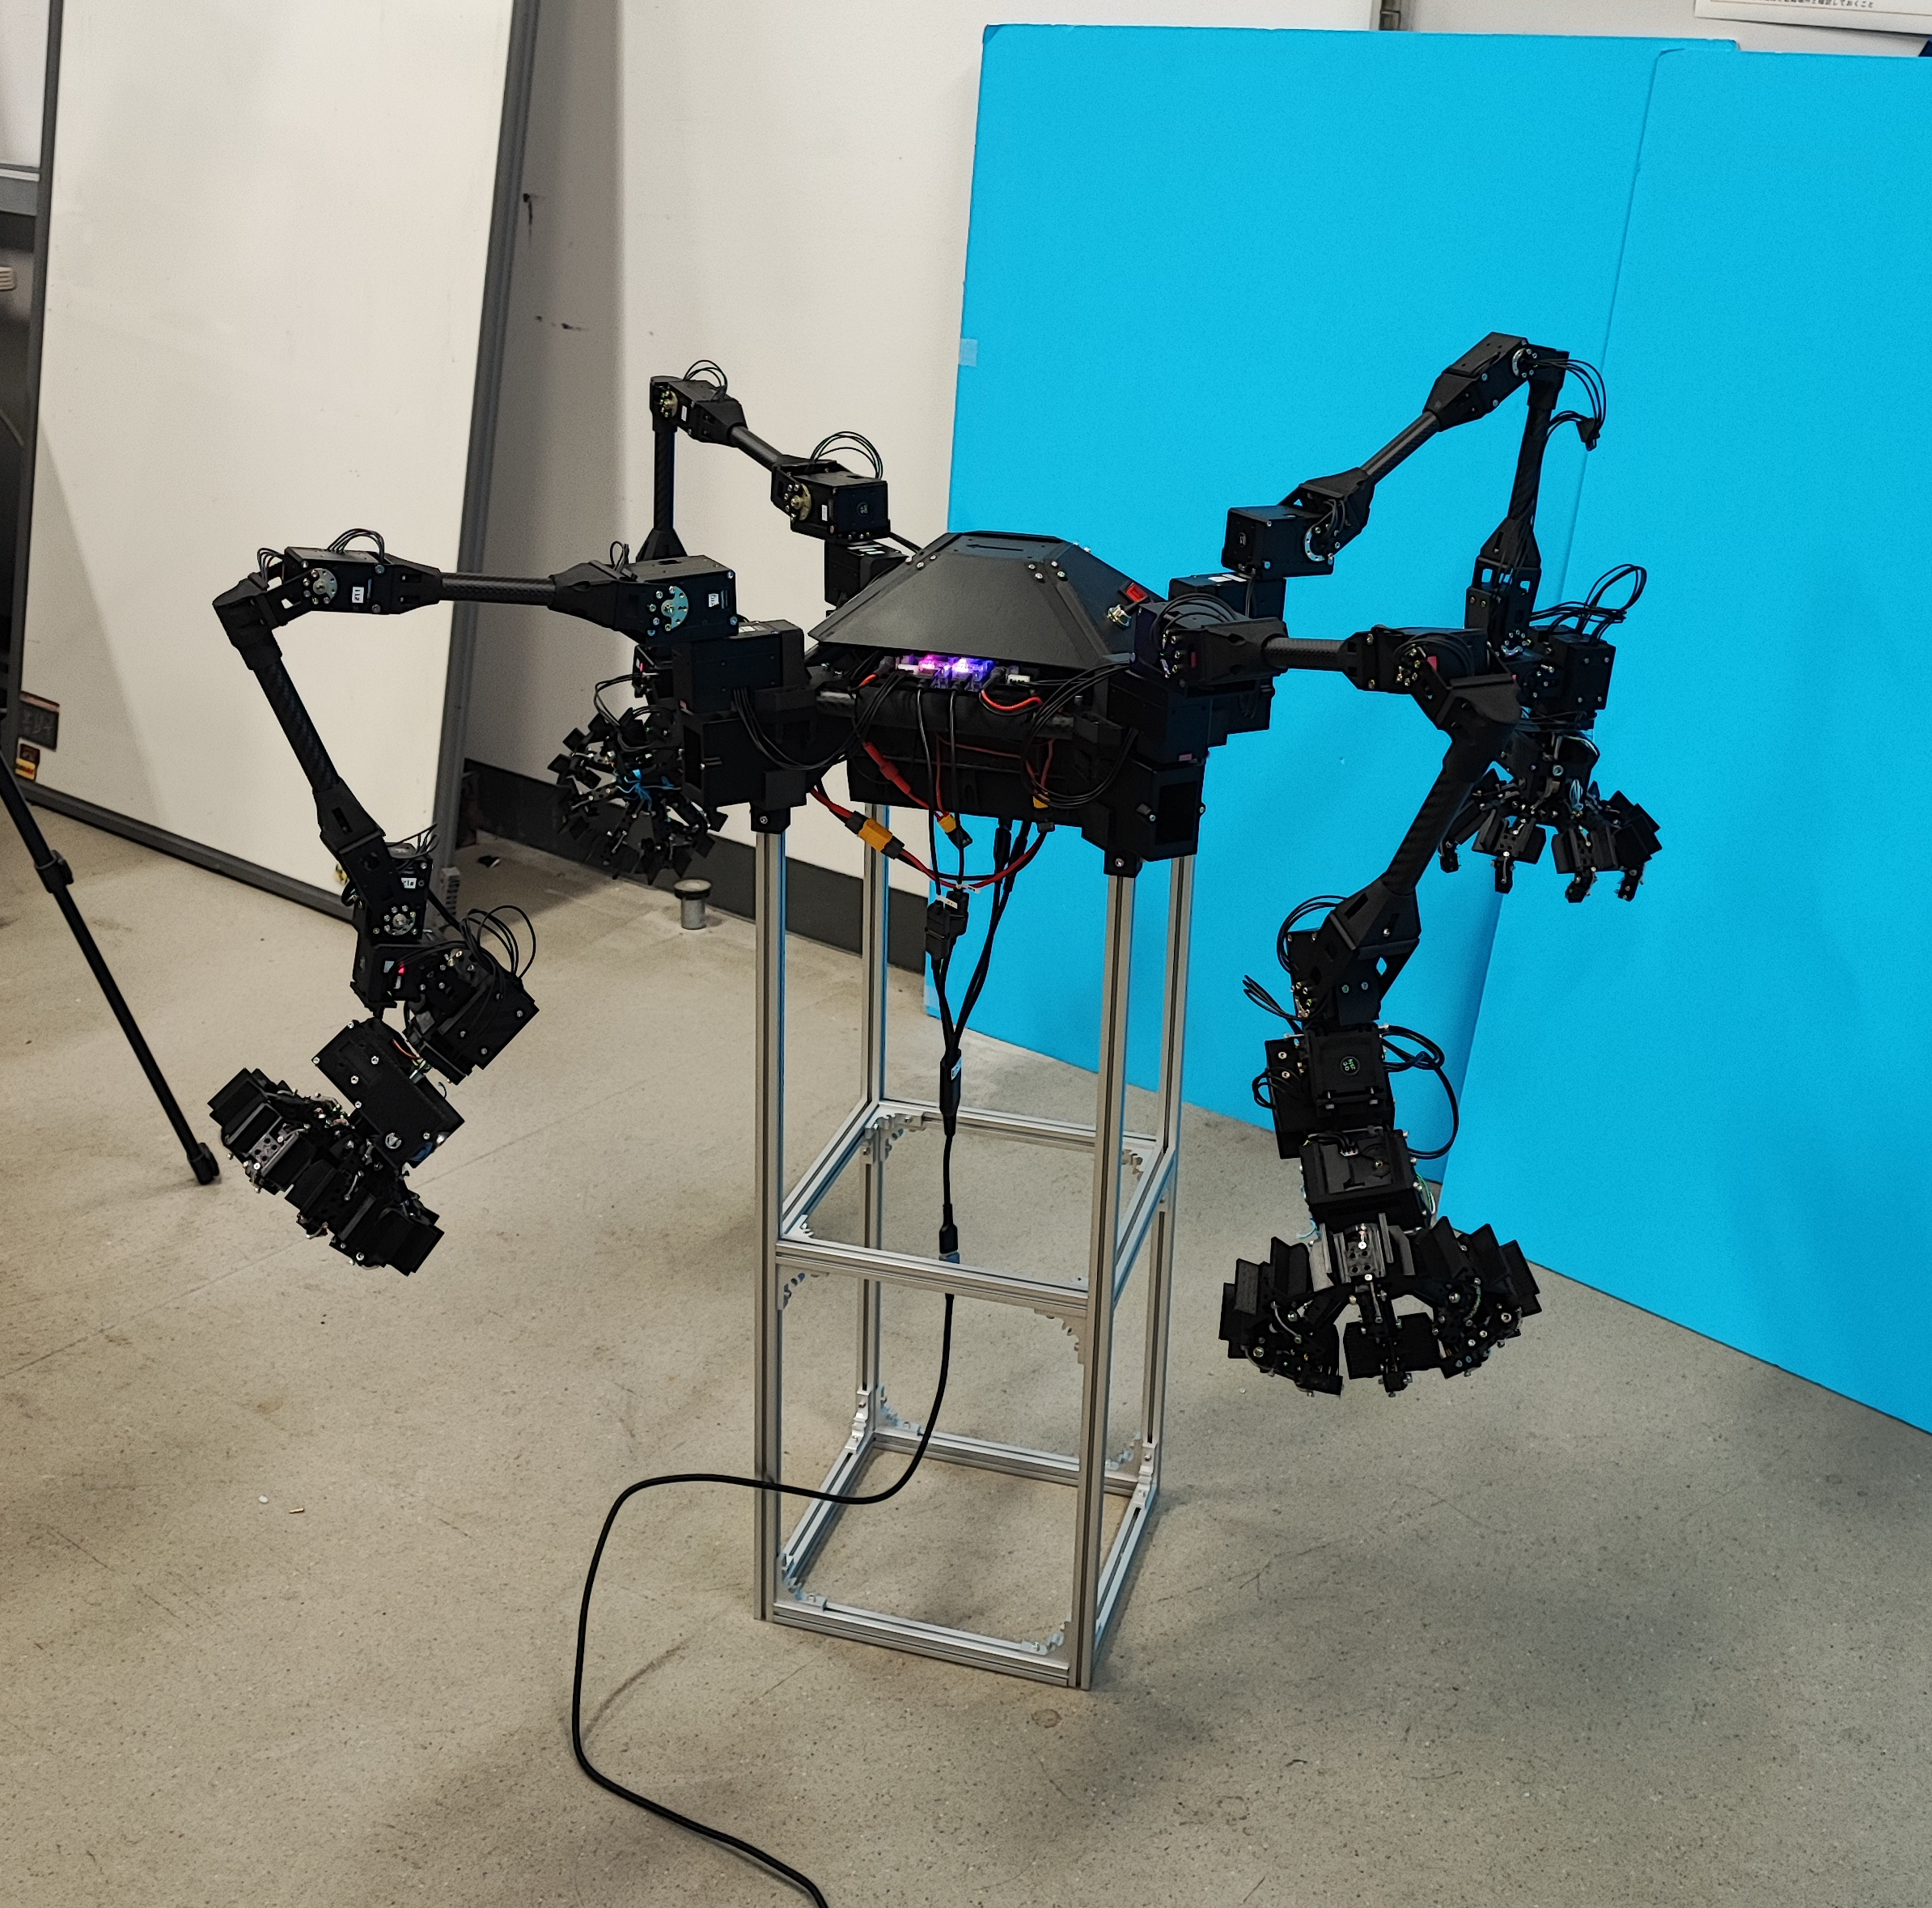
\includegraphics[width=0.5\textwidth]{Images/img_ch7/robot_testbench.jpg}
    \caption{Assembled LIMBERO-GRIEEL robot, supported for testing}
    \label{fig:robot_testbench}
\end{figure}


From these preliminary tests, especially (\ref{item:robot_test2}), the limitations on the shoulder (C2F) and elbow (F2T) joint's motor and design have been further proven. In addition, for some standing configurations, the $wristV$ joint is subjected to a big gravitational load, and the specification of the motor (as reported in \ref{table:DYNAMIXEL}) shows its limited rated torque. 
When subjected to excessive payload to hold joint position, DYNAMIXEL motors get overloaded/overheated, entering protection shutdown mode.

To solve the problem above, an empirical load compensation has been integrated into the testing environment. 
The lower gravity testbed \cite{climbing_testbench}\cite{LIMBEROTakadaThesis} used at the SRL was not available during the experiments, and an alternative solution has been employed. While the testbed includes an accurate counterweight gimbal mechanism to provide always a vertical force, here a simple but less accurate approach is used, attaching the frame of the robot base to a counterweight through a pulley, as schematized in Fig.\ref{fig:robot_testbench_counterweight}.
This system guarantees the base support but introduces additional disturbances that the motion control has to compensate for. 

\begin{figure}[H]
    \centering
    \subfloat[Vertical gravity compensation\label{fig:contact}]{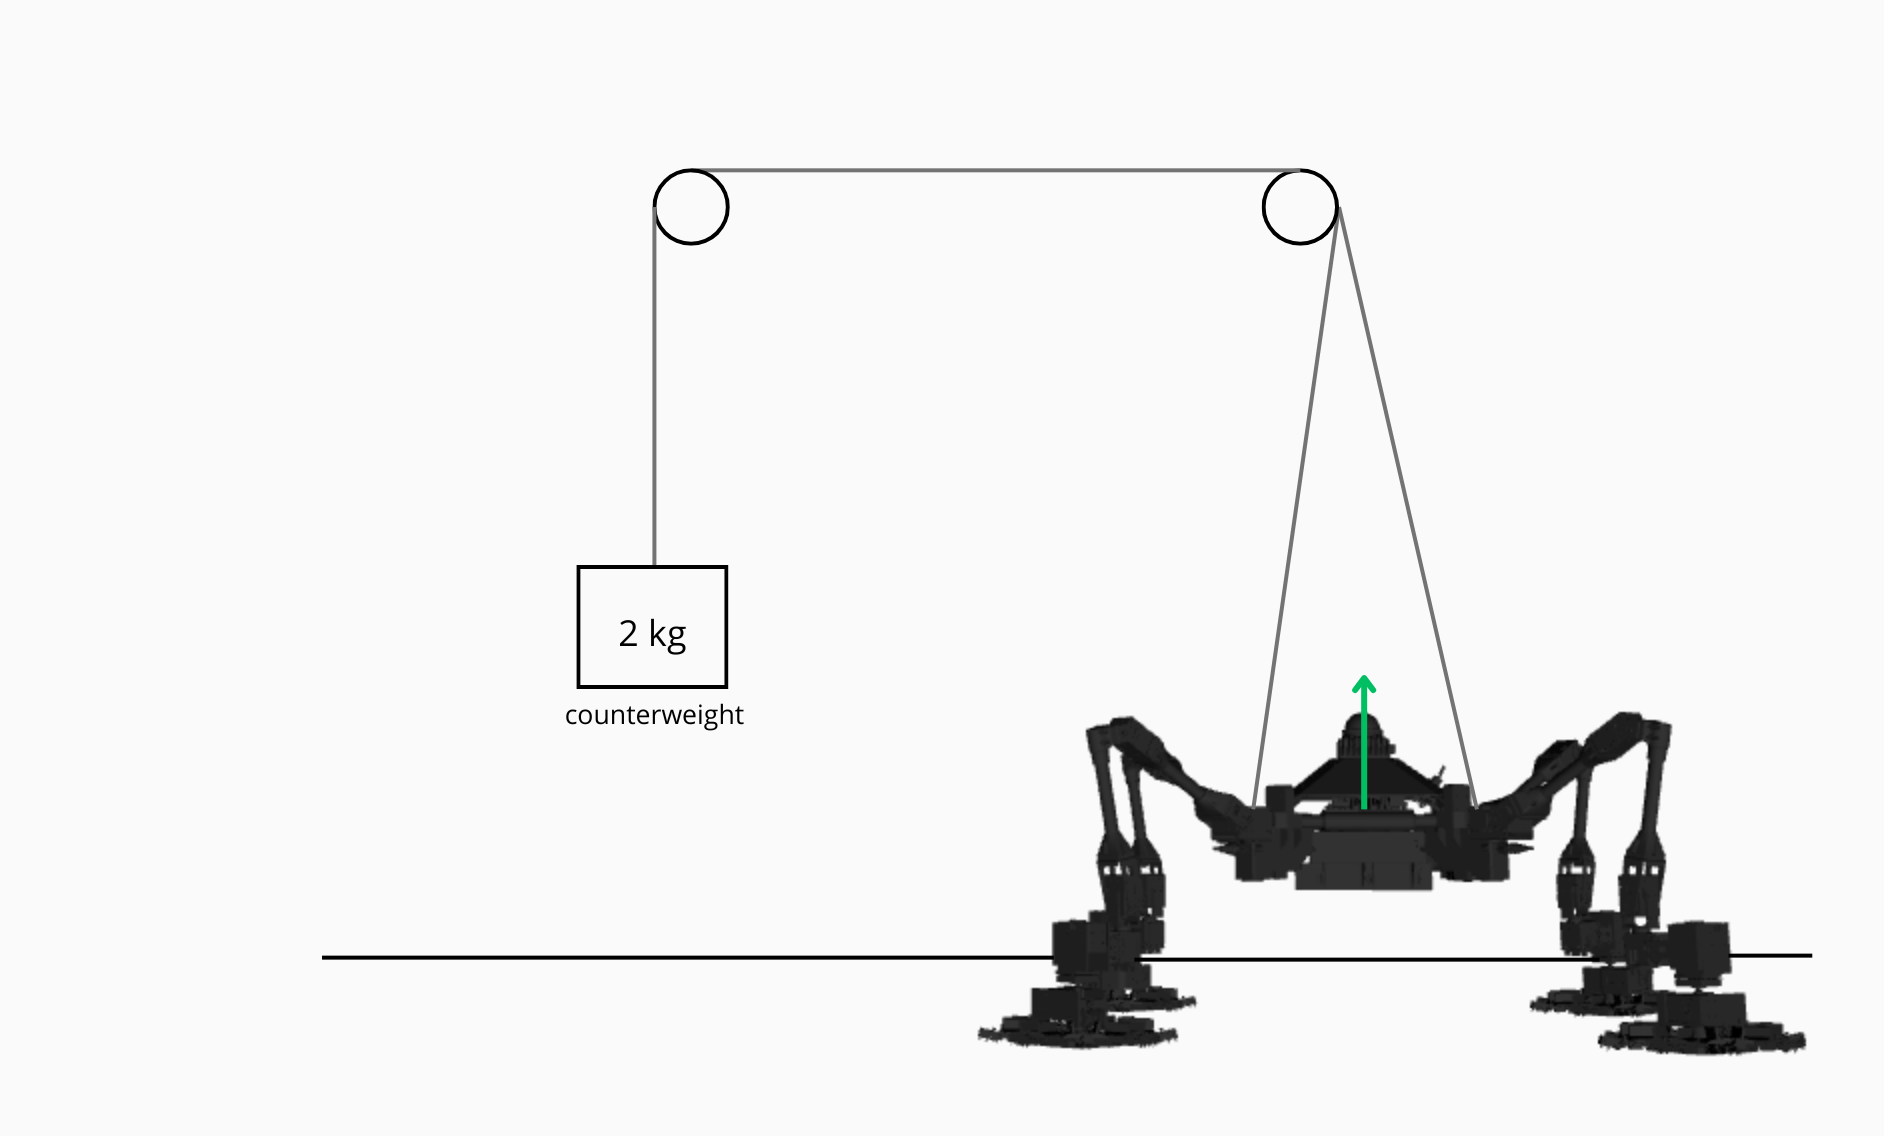
\includegraphics[width=0.46\textwidth]{Images/img_ch7/Vertical.png}} \quad 
    \subfloat[Inaccurate compensation, causing disturbances\label{fig:not_contact}]{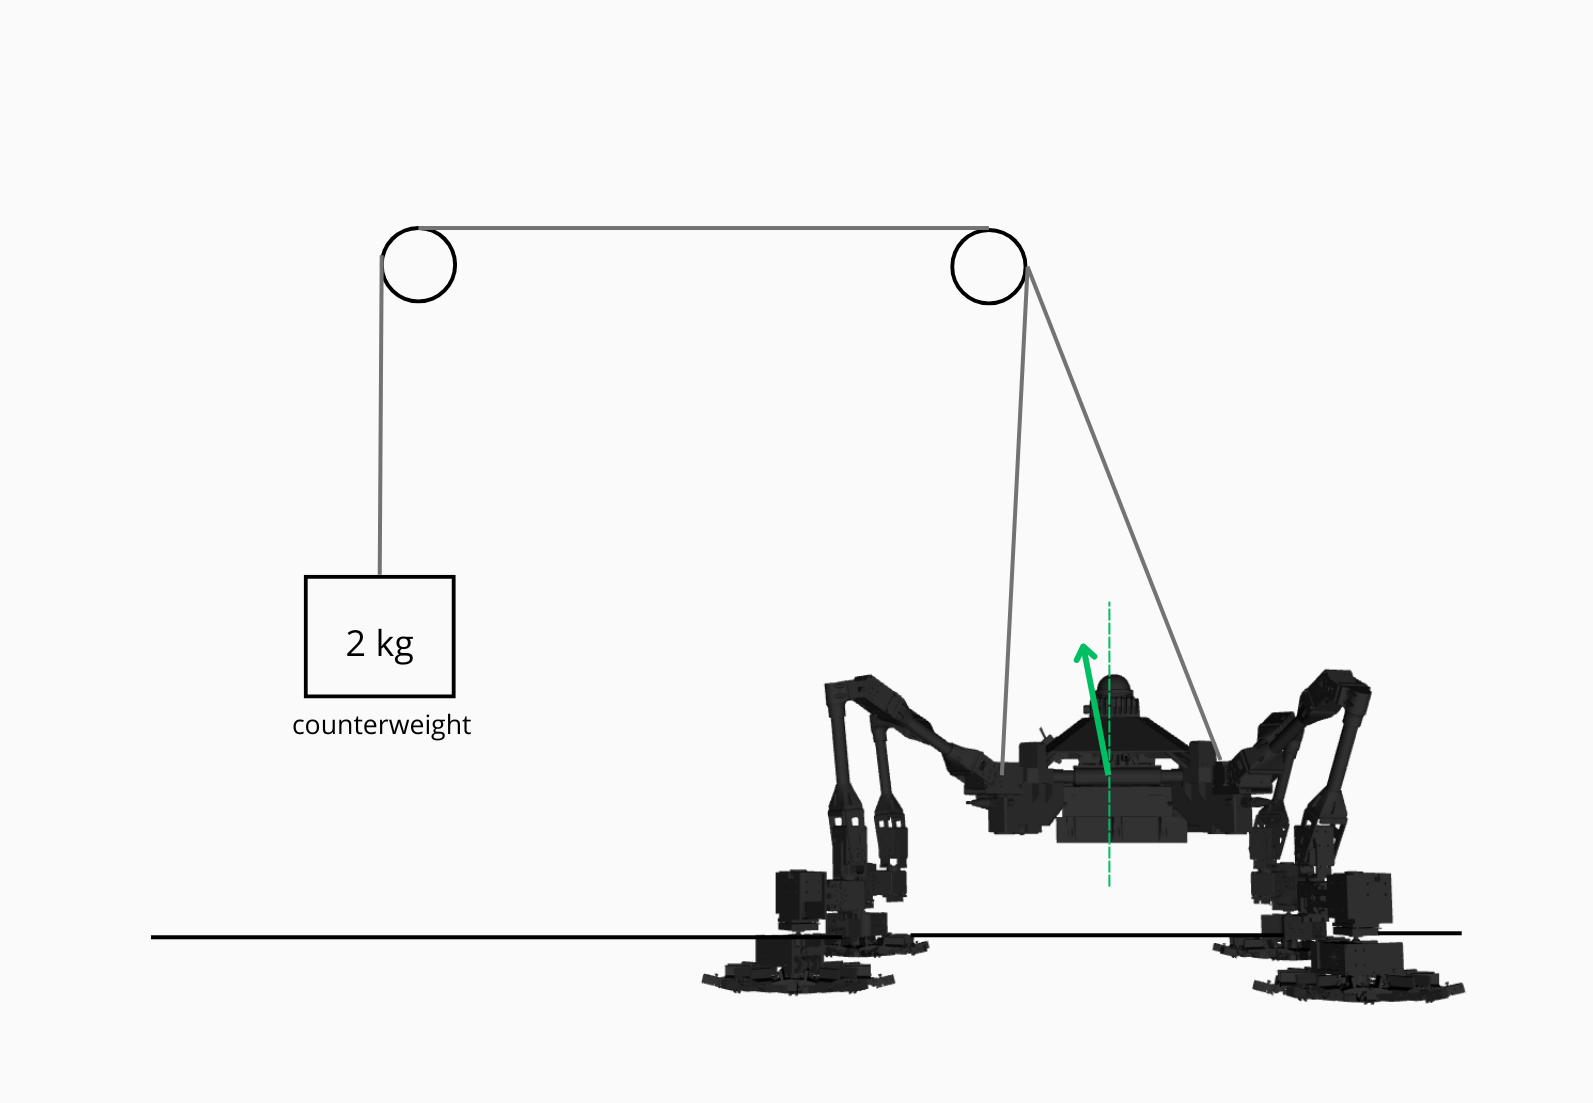
\includegraphics[width=0.4\textwidth]{Images/img_ch7/BadCounterweight.png}} 

    \caption[Empirical counterweight system for experiments]{Empirical counterweight system used in the experiments}
    \label{fig:robot_testbench_counterweight}
\end{figure}


Finally, when the limbs can support the base with the help of the counterweight solution described, the main experiments are carried out: 
\begin{enumerate}
    \setlength\itemsep{-0.7em} 
    \item\label{item:robot_exp1}\textbf{Motion tasks}: Verify that the motion control system executes single base and limb motion tasks with satisfactory performances. 
    \item\label{item:robot_exp2}\textbf{Single limb transformation}: Verify that single limb transformation can be completed with the motion sequence defined in Algorithm \ref{alg:single_grieel_transition}, ensuring stability margin. 
    \item\label{item:robot_exp3}\textbf{Locomotion transition}: Verify that the locomotion mode transformation algorithm (\ref{alg:multiple_grieel_transition}) is completed with satisfactory robot stability.  
\end{enumerate} 

